
\begin{table}[ht]
    \begin{center}
    \caption{Novel Composition}
    \label{novel_composition_table}
    \begin{tabular}{|p{2cm}|p{5cm}|}
    \hline
    \textbf{Name} & \textbf{Novel Combinations} \\
    \hline
    object-relationship & touching table, touching food, beneath table, beneath food\\
    \hline
    repetition & taking a dish from somewhere, putting some food somewhere\\
    \hline
    first/last & looking at first, behind first, holding first \\
    \hline
    before/after & before standing up, before playing with phone, before throwing broom\\
    \hline
    longer & longer than standing up, longer than playing with phone, longer than throwing broom\\
    \hline
    
    \end{tabular}
    
    \end{center}
\end{table}



\newpage

\begin{figure}[t]
\begin{center}
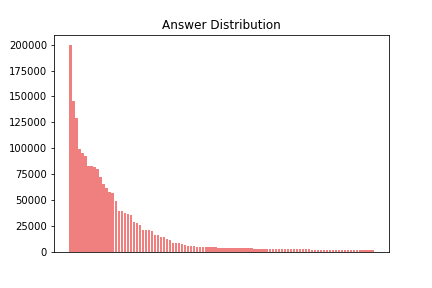
\includegraphics[width=0.8\linewidth]{Figures/answer_dist.png}
\end{center}
   \caption{The distribution of the top 100 answers (excluding "Yes" and "No").}
\label{answer_dist}
\end{figure}


\begin{figure}[t]
\begin{center}
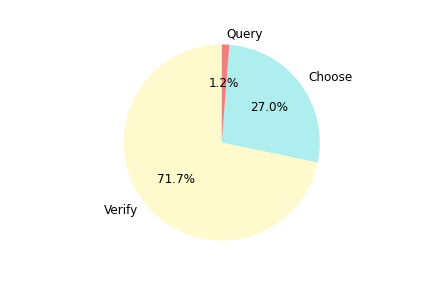
\includegraphics[width=0.8\linewidth]{Figures/struct_dist.png}
\caption{The structural distribution of questions.}
\end{center}
\label{structural}
\end{figure}


\begin{figure}[t]
\begin{center}
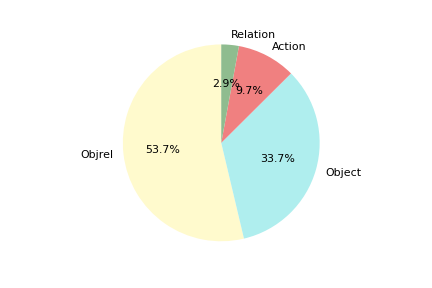
\includegraphics[width=0.8\linewidth]{Figures/sem_dist.png}
\end{center}
   \caption{The semantic distribution of questions.}
\label{semantics}
\end{figure}


\begin{figure}[t]
\begin{center}
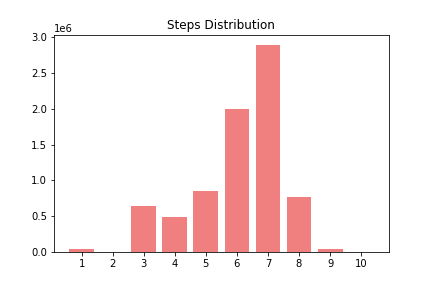
\includegraphics[width=0.8\linewidth]{Figures/steps_dist.png}
\end{center}
   \caption{The distribution of the number of compositional steps.}
\label{steps}
\end{figure}


\begin{figure}[t]
\begin{center}
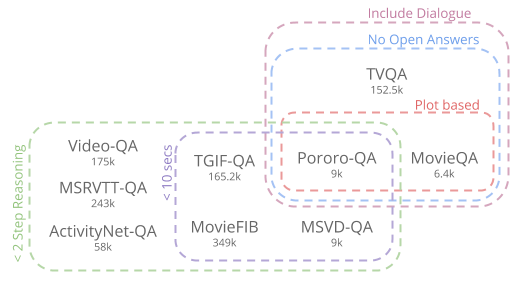
\includegraphics[width=0.8\linewidth]{Figures/figure_videoQA.png}
\end{center}
   \caption{Existing VideoQA benchmarks have some drawbacks. Specifically, many have questions with less than 2 steps of reasoning, using short videos, having plot based questions, only multiple choice questions, and including dialogue.}
\label{existing_benchmarks}
\end{figure}


\begin{figure}[t]
\begin{center}
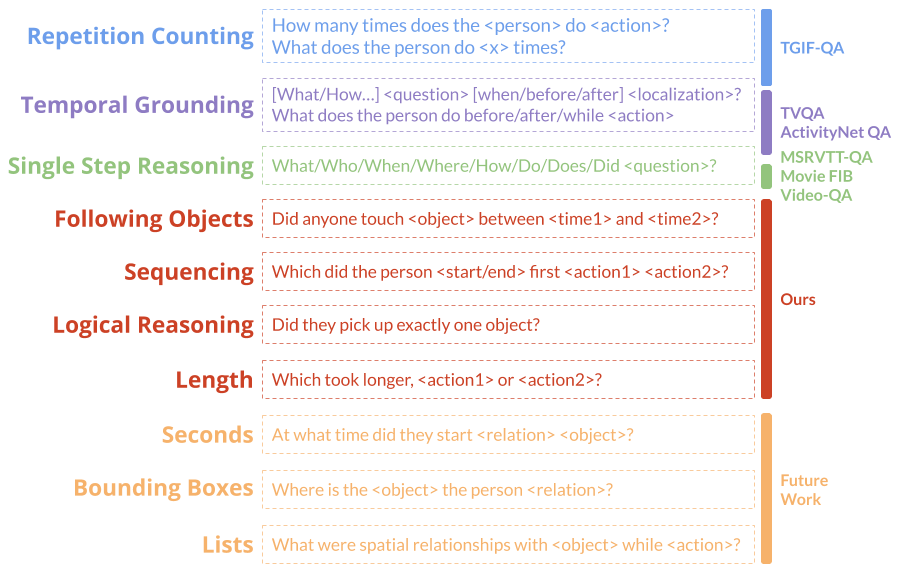
\includegraphics[width=0.8\linewidth]{Figures/figure_temporalTypes.png}
\end{center}
   \caption{Various types of temporal reasoning.}
\label{temporal_types}
\end{figure}


\begin{figure*}[t]
\begin{center}
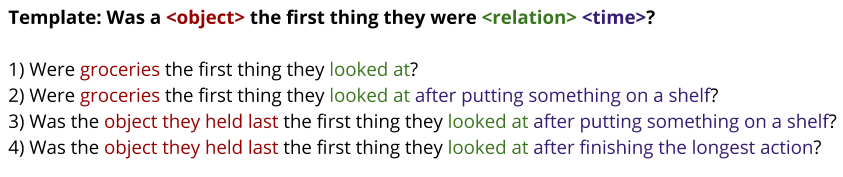
\includegraphics[width=0.8\linewidth]{Figures/figure_indirect.png}
\end{center}
   \caption{Our pipeline uses indirect references to create a variety of questions with different required reasoning steps from the same template. 1) uses all direct references and no temporalization. It has two steps of reasoning (determining if looked at groceries, then finding if that is the first thing at which they looked). 2) Adds temporal localization for a total of 4 steps (localizing when putting something on a shelf, then shifting attention after). 3) Uses an indirect reference for the object, adding one additional step (the last object held) for a total of 5 steps. 4) adds an indirect reference within the temporal localization to add a step (find the longest action) for a question with a total of 6 compositional steps required to answer.}
\label{template_expansion}
\end{figure*}

\begin{figure*}[t]
\begin{center}
%\fbox{\rule{0pt}{2in} \rule{.9\linewidth}{0pt}}
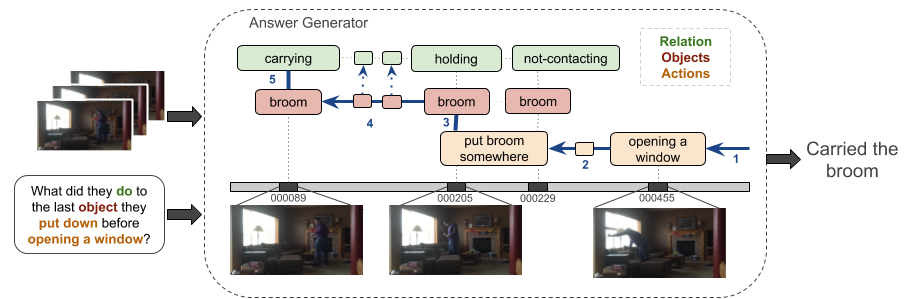
\includegraphics[width=0.8\linewidth]{Figures/figure_questionGenerator.png}
\end{center}
   \caption{The sequence in which our answer generator traverses the spatio-temporal scene graph to automatically generate the answer to a question. The input question can be decomposed into the following spatio-temporal operations: 
  1) localize when the actor opened a window, 
  2) find the last event before then when the actor put an object down, 
  3) determine which object (the broom) was put down, 
  4) look for a different relationship between the actor and this broom, 
  5) Output that the actor ``carried the broom''.}
\label{answer_generator}
\end{figure*}

\begin{figure}[t]
\begin{center}
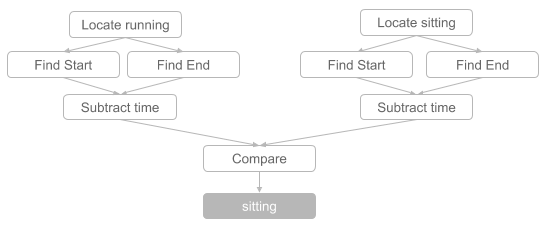
\includegraphics[width=0.8\linewidth]{Figures/figure_composition.png}
\end{center}
   \caption{The substeps required to answer the question "Was the person running or sitting for longer?"}
\label{compositional_substeps}
\end{figure}




%\begin{figure}[t]
%\begin{center}
%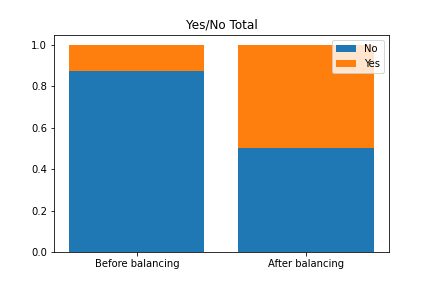
\includegraphics[width=0.8\linewidth]{Figures/yn_total.png}
%\end{center}
%   \caption{The proportion of questions with a Yes/No answer before and after balancing}
%\label{binary_balance}
%\end{figure}


\begin{table}[ht]
    \begin{center}
    \caption{Suite of Metrics}
    \label{metrics}
    \begin{tabular}{|p{2cm}|p{5cm}|}
     \hline
     \multicolumn{2}{|c|}{\textbf{Content Category}}\\
    \hline
    All & Accuracy on all questions\\
    \hline
    Question Type & Accuracy on each question category (e.g. Counting, Length, First, ...)\\
    \hline
    Answer Type & Accuracy on each answer category (e.g. binary, and open)\\
    \hline
    
    
     \multicolumn{2}{|c|}{\textbf{Generalization}}\\
    \hline
    Video Length & Train on videos of length $<$ 30 seconds. Test on videos of length $\geq$ 30 seconds \\
    \hline
    Actions & Train on videos with $<$ 5 actions. Test on videos with $\geq$ 5 actions  \\
    \hline
    Compositional Steps &  Train on questions with $<$ 6 steps. Test on questions with $\geq$ 6 steps  \\
    \hline
    Novel Compositions & See Table \ref{novel_composition_table} \\
    \hline
    Indirect Consistency & Accuracy on questions referring to the same ideas but using different numbers of indirect references\\
    \hline
    Direct Only & Questions with no indirect refs\\
    \hline
    \% Training Data & Train on only 1, 5, 10 and 20 percent of training data \\
    \hline
    
    
     \multicolumn{2}{|c|}{\textbf{Answer Legitimacy}}\\
    \hline
    Sequencing & Something where sequencing is consistent \\
    \hline
    Consistent & If answers a question correctly, answers all logical entailments correctly \\
    \hline
    Validity & Answer type is of correct genre (e.g. object, relation, action, count, yes/no)\\
    \hline
    Plausibility  & Answer exists in distribution for that question\\
    \hline
    Distribution & Predicted answers follow same distribution as ground truth\\
    \hline
    \end{tabular}
    \end{center}
\end{table}


\begin{table}[ht]
    \begin{center}
    \caption{Novel Composition}
    \label{novel_composition_table}
    \begin{tabular}{|p{2cm}|p{5cm}|}
    \hline
    \textbf{Name} & \textbf{Novel Combinations} \\
    \hline
    object-relationship & touching table, touching food, beneath table, beneath food\\
    \hline
    repetition & taking a dish from somewhere, putting some food somewhere\\
    \hline
    first/last & looking at first, behind first, holding first \\
    \hline
    before/after & before standing up, before playing with phone, before throwing broom\\
    \hline
    longer & longer than standing up, longer than playing with phone, longer than throwing broom\\
    \hline
    
    \end{tabular}
    
    \end{center}
\end{table}
